% TO DO
% Mise à jour des modifications de François
% Représentation schématisée du modèle
% Eq. 12: add the two coordinates in the text
% Vérifier la présence des chapeaux aux équations
% Relecture de l'ensemble du texte
% Rédaction de la discussion
% Rédaction du résumé
% TARGET: Am Nat ou Ecology

\documentclass[12pt]{article}
\usepackage[utf8]{inputenc}
\usepackage{color,dcolumn,graphicx,hyperref}
\usepackage{wrapfig}

\begin{document}

\title{How likely is speciation in neutral ecology ?}

\author{Philippe Desjardins-Proulx, Dominique Gravel}

% \begin{abstract} 
% Patterns of biodiversity predicted by the neutral theory rely on a simple
% phenomenological model of speciation. To further investigate the effect of
% speciation on neutral biodiversity, we analyze a spatially-explicit neutral
% model based on population genetics. We define the metacommunity as a system of
% populations exchanging migrants use this framework to introduce speciation with
% little or no gene flow (allopatric and parapatric speciation). We find that with
% realistic mutation rates, metacommunities driven only by neutral processes
% cannot support more than a few species. Adding natural selection in the
% population genetics of speciation increases the number of species in the
% metacommunities and generate patterns of species distribution similar to those
% predicted by Hubbell's neutral theory of biodiversity.
% \end{abstract}

%\keywords{Neutral theory, speciation, metacommunity, allopatry,
%parapatry, graph theory}

\maketitle

%========================================================%
\section{Introduction}

How patterns of biodiversity arise through ecological and evolutionary
processes is a central question in modern ecology. According to Hubbell's
neutral theory of biodiversity (NTB), patterns of biodiversity such as
species-abundance distributions can be explained by the balance between
speciation, dispersal and random extinction. The neutral theory provides a
good fit to species distribution curves, and it has been extended in several
ways. The neutral theory has been shown to be flexible enough to fit nearly
any distribution, but it is often regarded as a valid starting point and an
interesting null hypothesis for community ecology.

\begin{wrapfigure}{l}{0.5\textwidth}
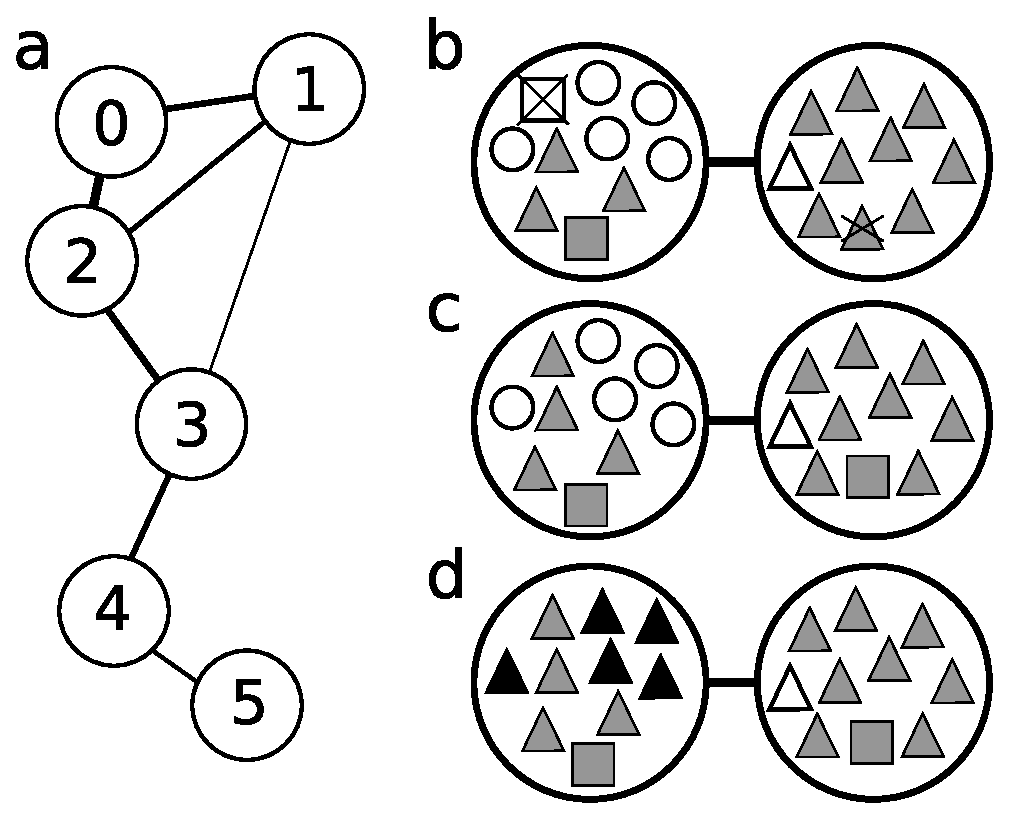
\includegraphics[width=0.35\textwidth]{fig.eps}
\caption{\textbf{The metacommunity as a graph of local communities. Each community is
connected by dispersal to one or more communities.}}
\vspace{-1em}  
\end{wrapfigure}

While a lot has been said about the assumption of ecological equivalence, much
less attention has been given to the speciation mode, which is sometime seen
as the theory's weakest point. In recent years, some studies altered the
speciation model within neutral ecology. However, nothing has been done to
relate the theory to population genetics and known models of speciation,
despite the fact that, as Etienne et al. noted, such a mechanistic model could
eventually force us to reject neutrality. The neutral theory with point
speciation has also been criticized for predicting too many rare species, too
many young species, and for assuming a direct relationship between abundance
and speciation. With random-fission, the neutral theory predicts less rare
species, but the resulting species abundance curves result in a worst fit.

In this article, we introduce a neutral theory of biodiversity with a
speciation model derived from population genetics. We emphasize the role of
allopatric and parapatric speciation. Speciation modes are most often
distinguished according to the level of gene flow between the diverging
populations. Allopatric speciation occurs when the new species originates from
a geographically isolated population. By contrast, sympatric speciation is
often defined as speciation without geographical isolation, in short, when the
diverging populations share the same location. Lastly, parapatric speciation
covers the middle ground between these two extremes.

In the original neutral theory's formulation, Hubbell presented two models of
speciation, point-speciation and random-fission speciation. Both are
phenomenological individual based models. In the case of point-speciation, a
newly recruited individual is selected at random and undergoes speciation. In
the case of random-fission, the whole species is divided in two at random. In
both cases, the probability of speciation of a given species is directly
proportional to abundance and independent of dispersal. Hubbell associates the
point-speciation model with sympatric speciation, and the random fission model
with allopatric speciation. Some rare forms of sympatric speciation are indeed
similar to the point speciation model, namely polyploid speciation, but most
sympatric speciation events involve a population being divided in two by non-
geographical factors. Also, as neither models take gene flow into
consideration, neither can distinguish sympatric and allopatric speciation
events.

%\begin{figure}
%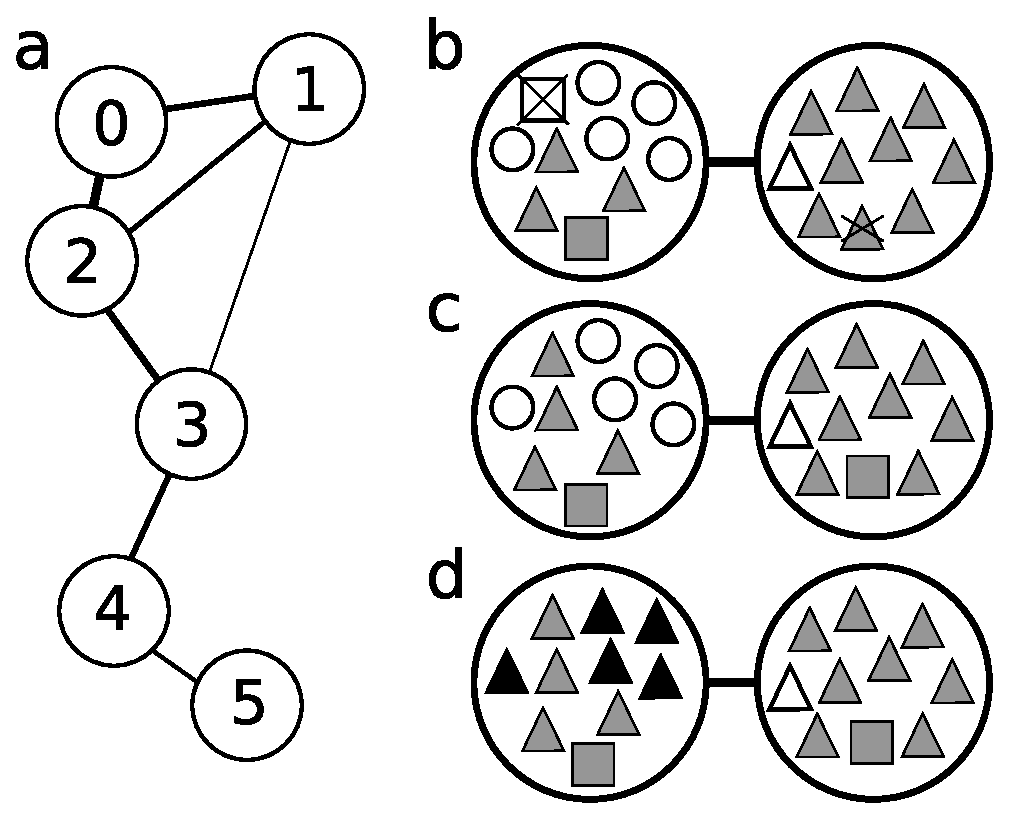
\includegraphics[width=0.35\textwidth]{fig.eps}
%\caption{The metacommunity as a graph of local communities. Each community is
%connected by dispersal to one or more communities.}
%\vspace{-1em}  
%\end{figure}

While theoretical models have shown sympatric speciation to be possible,
empirical studies have uncovered only a very few solid cases and much of the
theory is controversial. Despite the growing acceptance of sympatric
speciation as a plausible cause of speciation, most speciation events are
still thought to occur with limited gene flow. Allopatric and parapatric
speciation events are more common, but modelling them require some details
about the spatial structure of the metacommunity. We chose to base our model
on the most common forms of speciation despite the increased complexity of a
spatially-explicit framework. We find that with realistic parameters,
metacommunities cannot support more than a few species when the genetics of
speciation is assumed to be neutral. We also considered a simple alternative
pseudo-selection model by adding natural selection at the genetic level, but
keeping the ecological equivalence assumption at the individual level. This
approach shows that the rates of speciation typical of the NTB cannot be
obtained without selection pushing mutations to fixation.

\section{Model}

We model speciation with the Bateson-Dob\-zhan\-sky-Muller model (BDM) in
which reproductive isolation is the consequence of the accumulation of
incompatible alleles. While the BDM model is simple, we have many empirical
and theoretical reasons to believe that speciation events often follow a
similar scheme. We use a two-loci and two-alleles version of the model where
sexual reproduction is ignored. Each population starts with the $ab$ haplotype
fixed. The allele at the first locus, $a$, mutates to $A$, and the allele at
the second locus, $b$, mutates to $B$. Both mutates at the same rate $\mu$. We
follow Gavrilets and ignore back mutations. Alleles $a$ and $B$ are
incompatible, so the path from $ab$ and $AB$ can be seen as a process with
three states:

\end{document}
